\chapter{Algorithm Implementations}
\label{sec:chapterimplementation}
This chapter consists of implementing support for the standard geometry file formats, re-implementing the baseline, and descriptions of extensions that provide operability support for the baseline.

\section{WKT, WKB \& Gzip}
% Kort om våra första implementationer. Dessa jämförs ju inte sen då de är en invalid baseline. Men kan ändå vara bra att nämna lite
WKB is used as the reference when verifying the correctness of the implementations, and for size benchmarking, while WKT is convenient to use when debugging. Additionally, due to its smaller size and higher performance, WKB is commonly used in the industry. Therefore, classes utilizing Shapely for parsing and serializing WKT and WKB were written to support the benchmarking environment.
\\\\
Python includes support for working with most common compression formats, including the general-purpose formats \emph{gzip}, \emph{zlib}, and \emph{bzip2}. Classes consisting of serialization to WKB and WKT followed by compression using algorithms provided by the Python library were implemented in order to compare the compression ratios.


\section{Baseline: Floating-Point Delta}
\label{section:baseline}
As described in the related work section, floating-point delta (FPD) encoding is a compression algorithm suited for spatial data. Due to its simplicity while still being related to the spatial domain, the algorithm \cite{spatialparquet} serves as the baseline in this thesis.

Our implementation of FP-delta encoding, similar to \citeauthor{spatialparquet}'s implementation \emph{Spatial Parquet}, consists of one pre-iteration over the geometry in order to determine the optimal bit-length of the deltas, followed by interpreting the floating-point values as signed integers, and zigzag encoding the consecutive differences between the corresponding $(x, y)$ pairs. If either the x- or y-value overflows, a new chunk is created.

\begin{figure}[htbp]
    \centering
    \includesvg[width=15cm]{images/FP-Delta implementation.svg}
    \caption{Visualization overview of the bit structure of the FP-delta baseline format.}
    \label{img:fp_delta_base}
\end{figure}

Due to the differences between the underlying file formats, where Spatial Parquet is based on the Parquet standard, and the thesis on standalone files for each geometry, the encoding of the different geometry types differs between the implementations. The baseline format, as outlined in Figure \ref{img:fp_delta_base}, starts with two integers; the \textit{delta size} and the \textit{geometry type}, followed by a number of chunks that contain chunk metadata, required for parsing the geometry structure, and coordinate pairs. During parsing, the metadata is used to determine the context and length of the corresponding chunks, allowing for the reconstruction of the individual parts of the geometries. As also seen in the figure, the metadata differs between the geometry types and consists of:
\begin{itemize}
    \item \textbf{LineString}: the number of deltas in the current chunk.
    \item \textbf{Polygon}: + the number of chunks for the current ring.
    \item \textbf{MultiPolygon}: + the number of rings for the current polygon.
\end{itemize}

The geometric operations are implemented by decompressing the entire geometries, followed by executing either Shapely's built-in functions when it is sufficient to make a conclusion, or a self-made Python implementation of the operation. The latter is the approach utilized for \emph{Add Vertex}, \textit{Is Intersection} and \textit{Intersection}.


%\todo{byt namn på Chunk size till att det är antalet deltas som lagras, }


\section{Floating-Point Delta Extended}
In this section, we propose and implement enhancements to the geometric operations based on the FP-delta encoding. One motivation for the placement of the baseline's chunk metadata is to allow for further extension of the algorithm, enabling local decompression to improve the effectiveness of the operations. Throughout the report, our implementation is referred to as \emph{Floating-Point Delta Extended}, and abbreviated as \emph{FPDE}. Some of the ideas proposed below were not implemented due to time constraints, but may be of interest when conducting future research; they are marked with an asterisk (*) in the title of the section and can be skipped if the reader is only interested in the implemented concepts.

\subsection{High-Level Structure of the Format}
% Parsing data
% Chunk concept
% How are deltas encoded/decoded (chain)

\begin{figure}[htbp]
    \centering
    \includesvg[width=17.5cm]{images/fpde.svg}
    \caption{Visualization of the implemented structure for our solution. Extending the structure in Figure \ref{img:fp_delta_base}.}
    \label{img:fpde_structure}
\end{figure}

The final structure of the compression format, as seen in Figure \ref{img:fpde_structure}, is similar to the baseline, but both the global and chunk headers have been extended to allow for compressed computation. In summary, the implementation consists of a global header including the \emph{delta size}, \emph{geometry type}, \emph{entropy coding parameter}, \emph{chunk count}, \emph{chunk bounding boxes}, and the \emph{shape bounding box}. The global header is then followed by a sequence of chunks, where the chunk headers as previously contain the parsing data. If entropy encoding is applied, the size of each delta may vary, and to allow for skipping of irrelevant chunks, the total number of bits in each chunk is stored in the chunk header.

\begin{figure}[htbp]
    \centering
    \hspace*{0.5cm} 
    \includesvg[width=15.2cm]{images/flow_chart.svg}
    \caption{High-level flow chart of the compression and decompression operations in FPDE.}
    \label{fig:flow_chart}
\end{figure}


A high-level flow chart is presented in Figure \ref{fig:flow_chart} below, illustrating the sequential steps involved in the compression and decompression operations of the format. As for the baseline, the resulting size of different delta bit-lengths are calculated and the size optimal bit-length is assigned to the shape during compression. Two examples of how the resulting shape size varies with the delta bit-length can be seen in Figure \ref{fig:preiteration}. The chunk bounding boxes, required for the optimized intersection operations, and the global bounding box are calculated during compression. In addition, a maximum chunk size, which forces the creation of a new chunk when a certain number of deltas have been reached, can be specified as a configuration variable. As also visible in the flow chart, the format can configured to use one of three different floating-point encoding techniques, which are explained later in Section \ref{sec:delta_mod}.

\begin{figure}[htbp]%
    \centering
    \subfloat[\centering Shape from \emph{Sweden All}.]{{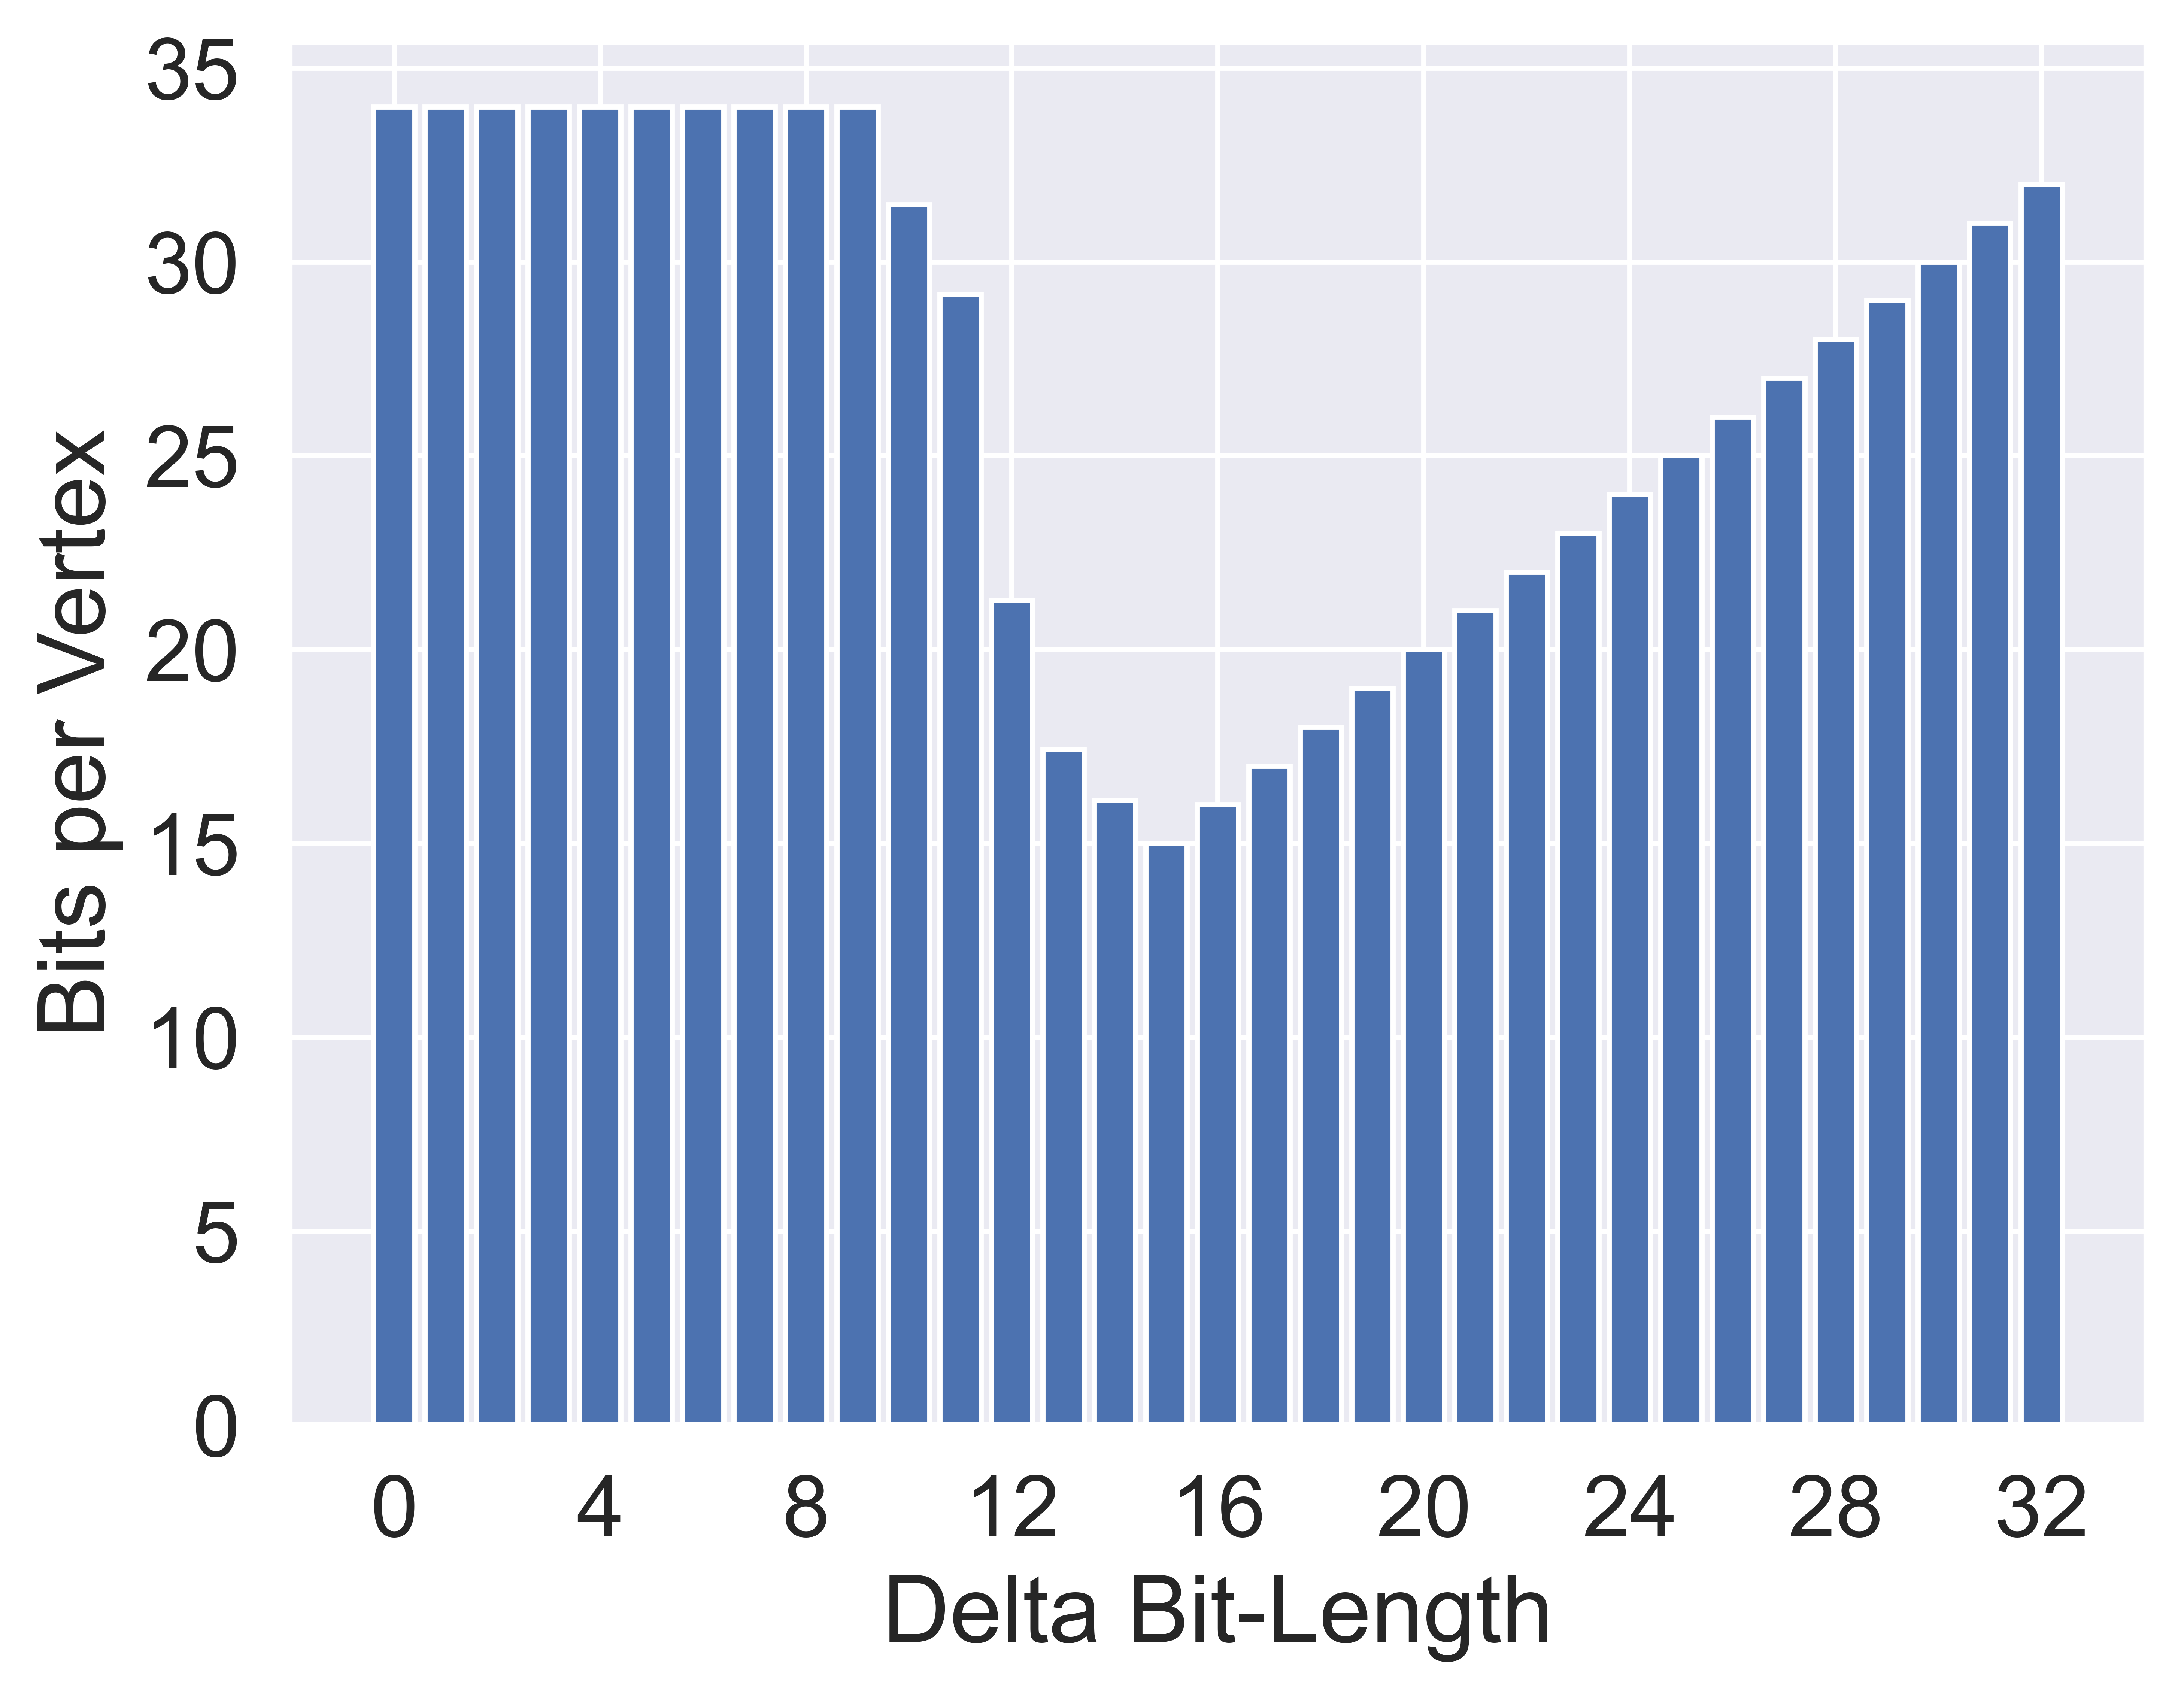
\includegraphics[width=6.9cm]{images/total_size_per_bit_size_sweden.png} }}%
    \qquad
    \subfloat[\centering  Shape from \emph{Admin Borders}.]{{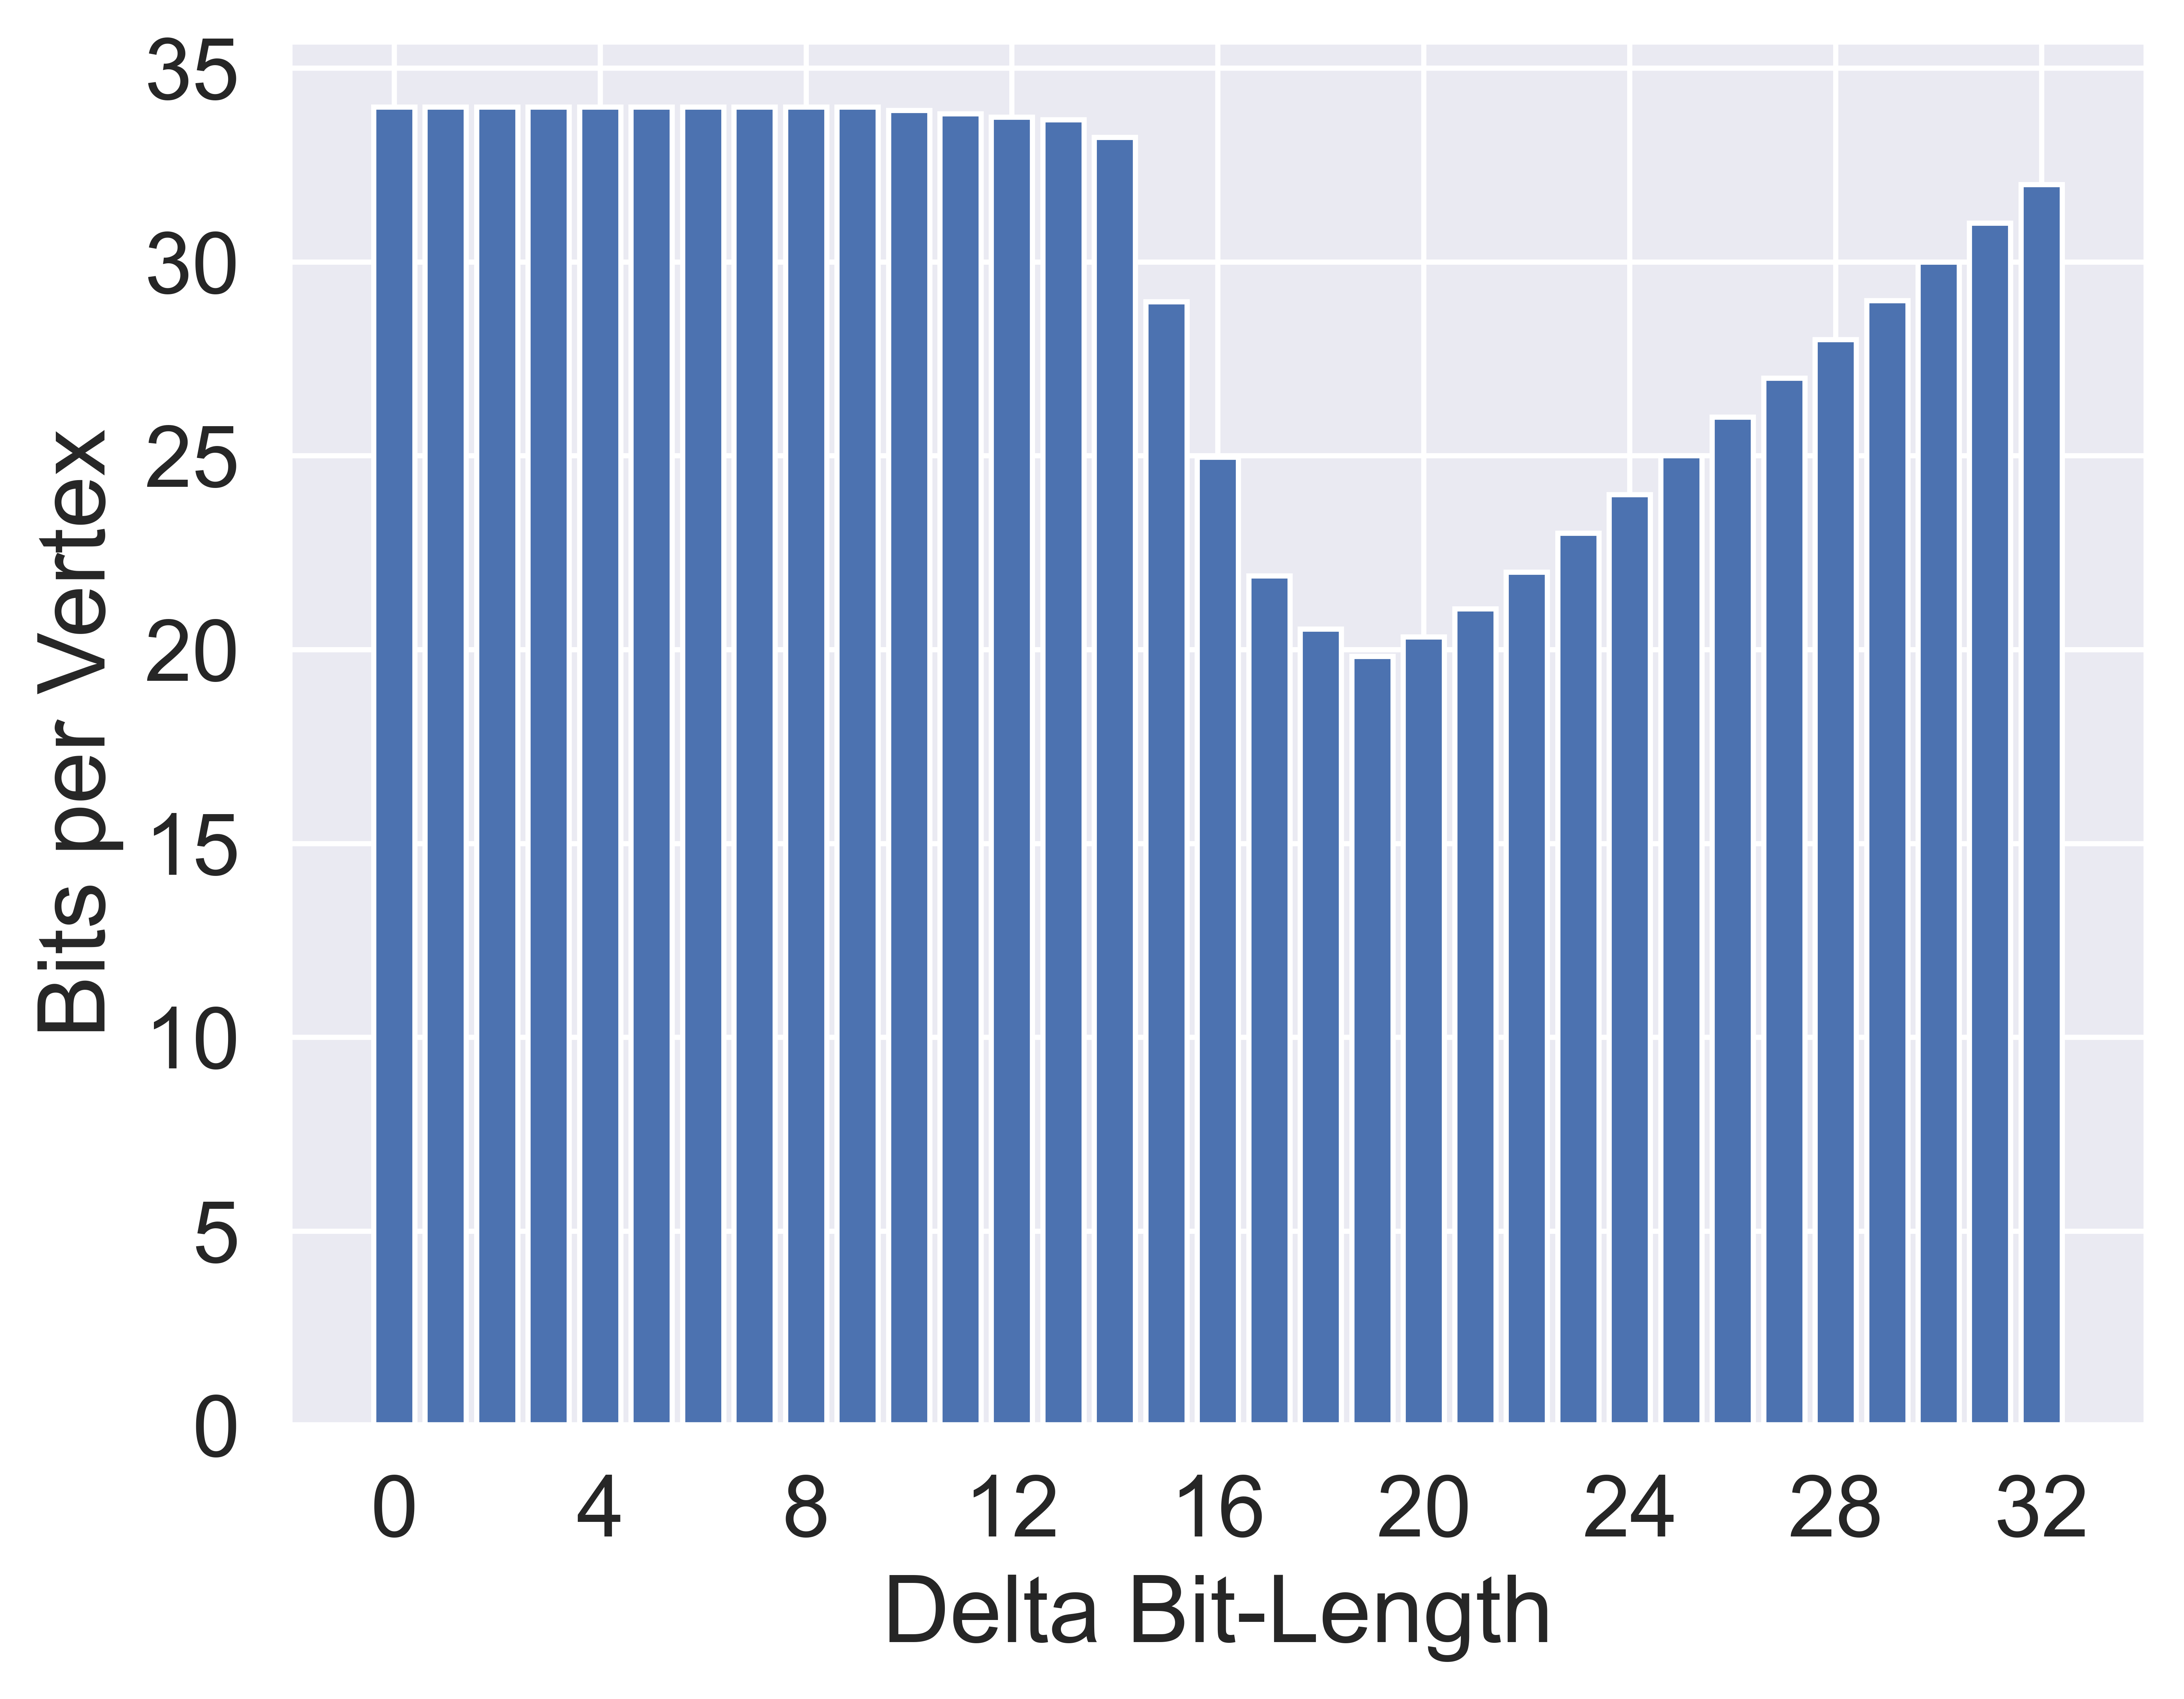
\includegraphics[width=6.9cm]{images/total_size_per_bit_size_world.png} }}%
    \caption{Combined size of all coordinates and chunk headers divided by the vertex count for different delta bit sizes. The figures show the data for two random geometries.}%
    \label{fig:preiteration}%
\end{figure}


% Baseline: Presentera statistik om data, diagram ex. Antal vertices
% Mätningar på vad som tar tid och plats
\section{Bounding Box}\label{boundingbox}
\begin{figure}[htbp]
    \centering
    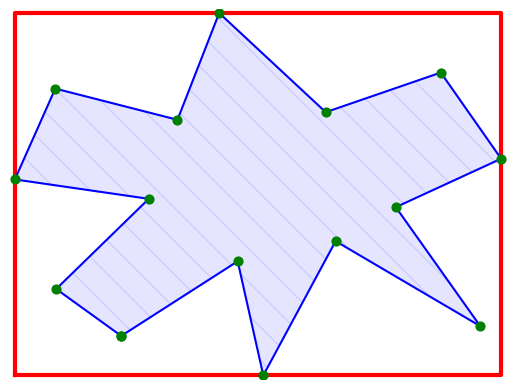
\includegraphics[width=5cm]{images/bbox_example.png}
    \caption{The red rectangle is the bounding box of the shape.}
    \label{fig:bboxexample}
\end{figure}

The minimal axis-aligned rectangle such that all points within the shape are contained is commonly referred to as the \emph{bounding box}. The bounding box can be used as a first step to filter out candidates for further operations. Since all points belonging to the shape are per definition within the bounding box, it can be used as a spatial upper bound for approximating the shape, implying that the shape is at maximum as large as the bounding box. For instance, the intersection operation can be optimized if there is no intersection between the bounding boxes, since this implies that no intersection can possibly occur between the shapes. An example of a bounding box can be seen in Figure \ref{fig:bboxexample}. 

Due to the bounding boxes commonly being used as a first filtration step, it is of great importance that the latency for fetching the bounding box is the lowest possible. Below, a number of implementations for storing and retrieving the bounding boxes are proposed. In FPDE, only the first approach is implemented and evaluated (Section \ref{sec:bboxfull}).

\subsection{Store Full Coordinates}\label{sec:bboxfull}
The first approach is to pre-compute the bounding box and store the bounds, essentially storing two diagonal corner points of the box, resulting in a total of four coordinates. As seen in Equation \ref{eq:bbmeta}, the coordinates of the bounding box are calculated by finding the minimum and maximum values of the X- and Y-vectors of the shape's vertices.
\begin{equation}
    bounds(s)=[\min(xs(s)),\ \max(xs(s)),\ \min(ys(s)),\ \max(ys(s))] = [x_l,\ x_r,\ y_b,\ y_t]
    \label{eq:bbmeta}
\end{equation}

The added overhead from the four coordinates results in a total space of $4 \cdot b_f$ where $b_f$ is the number of bits required to store one coordinate. The value of $b_f$ depends on the format used for serialization of the floating-point coordinates. If using double-precision, the resulting size is $4 \cdot 64 = 256$ bits.

Since the coordinates are stored in full, obtaining the actual bounding box from the memory address can be done in $\mathcal{O}(1)$.

\starsubsection{Store Indices for Spanning Points}
As seen in Equation \ref{eq:bbmeta}, the bounds are defined by a maximum of four unique vertices spanning the bounding box. Instead of storing the full coordinates separately, the overhead can be reduced by storing the indices of the vertices, resulting in Equation \ref{eq:bbind}.
\begin{equation}
    \label{eq:bbind}
    \begin{gathered}
    bounds(s)=[\arg \min(xs(s)),\ \arg \max(xs(s)),\ \arg \min(ys(s)),\ \arg \max(ys(s))] \\
    = [i_{xl},\ i_{xr},\ i_{yb},\ i_{yt}]
    \end{gathered}
\end{equation}
The bounding box can be calculated by retrieving the points based on the indices and taking the $x$- or $y$-coordinate based on the position within the bounds data.

This approach usually requires less space compared to storing the full coordinates, but has a slower query time. To store the indices $4 \cdot \lceil \log_2(V) \rceil$ bits are required. Meaning that with a larger number of vertices, more bits are required. Calculating the bounding box can be done in 
$4 \cdot T(random\_access)$ operations.

\starsubsection{Utilize Sorted List}
If the compressed shape's data structure already includes two lists with indexes or coordinates sorted by x- and y-values, the bounding box can be easily retrieved. Obviously, the sorted lists should not be included for the bounding box alone, but some other operations, such as the first method presented for intersection in Section \ref{sec:intersection}, require sorting.

In this case, no \emph{additional} overhead is added, and if the sorted lists contain indices, retrieving the actual bounding box can be done in $4 \cdot T(random\_access)$ operations. If the sorted lists contain delta encoded coordinates, the time complexity becomes $2 \cdot \mathcal{O}(1) + 2 \cdot T(random\_access)$; where the accesses to $x_l$ and $y_b$ are constant, since they are stored in full at the very beginning of the sorted lists. For $x_r$ and $y_t$, which are stored at the very end of the lists, the accesses are the worst-case for random access. In this case, the access has to loop over all chunk headers and decompress the entire final chunk. Resulting in $T(random\_access) = c_s + m_c$, where $c_s$ is the number of chunks, and $m_c$ is the number of deltas within the last chunk. An improved approach for random access is discussed in Section \ref{sec:optrandom}. 

\starsubsection{Quadtree Approximation}
\label{sec:quadtreeapproximation}
If the exact bounding box is not required, storing it directly can be avoided by using a quadtree. In this case, each bounding box in a set of bounding boxes is part of one of the nodes within the tree. Namely, the node with the largest depth such that the bounding box is fully contained within the quadrant. In libraries for storing and retrieving geometries, spatial indexing commonly uses a tree-like structure based on the bounding boxes of the shapes \cite{spatialindexing}. In such cases, it may be possible to retrieve which quadrant the shape is assigned to from the library. The bounds of the quadrant can then be used as the bounding box approximation.

As this thesis focuses on singular geometries, no spatial indexing is available for the shapes. However, Section \ref{sec:quadtreechunk} proposes a method to reduce the query time and data overhead of operations by employing a quadtree. In this approach, the quadtree approximation of the bounding boxes of the individual chunks within a shape is used, as opposed to storing the coordinates of all the chunks' bounding boxes in full.

% Används i andra operationer, bör vara snabb
% 1.Lagra koordinater för sig
% 2.Lagra index till koordinater som spänner bounding boxen
% 4.Quadtree approximation
% 3.Sorted lista av koordinater: behöver spara winding order

\section{Add Vertex}
In this thesis, \emph{Add Vertex} refers to the operation of inserting a point at a specific index in the shape, with a binary string as output. This represents the operation in \ref{eq:add_vertex_op}:
\begin{equation}
    Add\_Vertex(\emph{bin}_{\emph{in}},\ \emph{idx},\ \emph{point}) \xrightarrow{output} \emph{bin}_{\emph{res}} 
    \label{eq:add_vertex_op}
\end{equation}

\subsection{Indexing Scheme}
For shapes representing at least one polygon, simply using the vertex's index to determine the location of the new vertex can result in ambiguities. Two problems cause the ambiguities to arise:
\begin{enumerate}
    \item Irregular standards regarding if the first point should be equal to the last point in each ring, such that the coordinates form a closed path. Otherwise, the last line segment in each ring is formed implicitly.
    \item Between two rings, it is not clear whether the index is a part of the predecessor- or the successor ring.
\end{enumerate}
Add Vertex is implemented with rules such that a point can be inserted anywhere in the shape, but it is not possible to extend the shape with new rings or polygons. In theory, this can be solved by having separate operations \emph{Add Ring} and \emph{Add Polygon}, or extending the indexing scheme further. Implementation-wise, the ideas are very similar.

The indexing scheme used assumes:
\begin{itemize}
    \item The start- and endpoint is only represented by the first vertex in the ring. 
    \item After the last vertex of a ring, an additional "ghost"-index exists in order to allow for insertion at the end of a ring.
\end{itemize}

\subsection{Random Access \& Chunk Iteration}
\label{Random_access}

Random access is essential in order to implement the addition of vertices. In this sense, random access is the operation of retrieving a subset of the data, based on an indexing parameter. For adding a vertex, both the surrounding context, such as neighboring points and chunk headers, along with the data offset in the binary string corresponding to the insertion index, is needed for the operation.
\\\\
One way to achieve faster random access querying is through the avoidance of reading unrelated data. Additionally, when dealing with compressed data, decompression involves further operations which should be avoided when possible.

Conveniently, the chunks in FPD are isolated, and the only required information in order to parse a chunk is the location (offset) of its header. Furthermore, the sequential encoding ensures that each chunk contains a contiguous slice of the index vector. It is therefore trivial to check whether a chunk contains an index by checking if the index is within the chunk bounds, as shown in Equation \ref{eq:addvinchunk}.

\begin{equation}
contains\_index(i,\ c) = \begin{cases}c \leq i \leq c + m_c + 1, & \text { if } last\_chunk\_in\_ring(c) \\ c \leq i \leq c + m_c, & \text { otherwise }\end{cases}
\label{eq:addvinchunk}
\end{equation}

where $c$ is the index of the first vertex in the chunk, and $m_c$ is the number of deltas within the chunk.

Using the function above, it is possible to avoid reading and decoding irrelevant chunks. Instead, only the chunk header is read and the delta count is extracted. Then, the index bounds check is performed, and if the chunk is irrelevant, jumping to the next chunk and ignoring the deltas within the current chunk is done by adding $m_c \cdot 2 \cdot delta\_size$ to the data offset variable. This process is further illustrated by the second jump in Figure \ref{img:addvertex}.

In addition, the implementation employs caching based on \emph{temporal locality}, stating that recently accessed data will likely be accessed again soon. By storing the accessed chunks dynamically in memory, each chunk and vertex is only retrieved once for a complete query. For example, intersection usually involves multiple random access calls, and can benefit from caching. This is however unrelated to adding a vertex, since a complete query only accesses each chunk once.

\subsection{Insertion Procedure for the General Case}
In order to combat possible special cases, a general suboptimal approach in terms of size is used to insert the vertices. In this section, the general procedure is described, and possible improvements are listed in the following section.

\begin{figure}[htbp]
    \centering
    \includesvg[width=440pt]{images/add_vertex_fig.svg}
    \caption{An illustration of adding a vertex at index 6, while exploiting the locality of indexing within chunks.}
    \label{img:addvertex}
\end{figure}

Conceptually, the idea of the insertion procedure is to split the chunk currently containing the vertex corresponding to the insertion index into two chunks, along with placing the inserted vertex into an additional chunk. The existing chunk will therefore contain the left part of the previous chunk, followed by a new chunk containing only the added vertex, and an additional new chunk containing the right part of the old chunk.  

First, the offset pointer to the chunk currently containing the corresponding vertex is found using the random access method described above, and the data offset location of the corresponding vertex is calculated. A new chunk, containing only the new vertex, is created and inserted at the old vertex's offset. The predecessor (left) chunk and the successor vertex are altered in order to preserve the neighboring vertices.


The procedure is illustrated in Figure \ref{img:addvertex}. In detail, the restoration of the structure for the neighboring vertices is done by additionally examining:
\begin{itemize}
    \item If there are vertices to the left of the inserted chunk, i.e. the insertion caused the surrounding chunk to be split, then the count of deltas in the predecessor chunk is updated to only include the deltas to the left of the insertion point.
    \item If there are vertices to the right of the inserted chunk, an additional chunk is created to the right, and the vertex immediately after the inserted vertex becomes the reset point for the new chunk.  
\end{itemize}

Additionally, the ring header, i.e., the integer containing the number of chunks for the ring, has to be updated to account for the added chunks.

%// Navigera ti, i.e. the ll rätt chunk, hoppa
%// Lösning för att lägga till i det generella fallet
%// Hantering av specialfall samt varför dessa bör hanteras


\starsubsection{Merging the Created Chunks}
The algorithm works in the general case, however it is not optimal in terms of size. In most cases, two additional chunks are created, resulting in a larger overhead and the avoidance of delta encoding. When handling the left and right part of the old chunk, the creation of additional chunks can be avoided:
\begin{itemize}
    \item If the delta between the inserted point and its predecessor point is smaller than the maximum delta size, then let the new point be a part of the left chunk instead of creating the middle chunk.
    \item If the delta between the inserted point and its successor is smaller than the maximum delta size, then let the new point be a reset point for the right part of the old chunk instead of creating an additional right chunk.
\end{itemize}

Additionally, if a point is inserted at the end of an existing chunk, it may be possible to merge the two existing neighboring chunks into one. This is only possible if the distance between the inserted vertex and the two chunks is less than the maximum delta size, so that the new point bridges the current gap between the chunks.


The benefits of the optimizations are greater when the geometry has repeated adds, since in the limit the unoptimized implementation will result in all vertices being in their own chunks, i.e., all coordinates are represented in full. FPDE does not currently implement merging of the chunks, but implementing the proposed solutions should be straightforward.

\starsubsection{Improving Random Access}\label{sec:optrandom}
%Currently: $T(random\_access) = c_s \cdot m_c$
An efficient structure for random access would allow for access to the requested data section in constant time. In the format proposed above, the relevant chunk is first found through iteration over the chunk headers, and then the chunk is decompressed until the requested vertex is obtained. Therefore, requesting a vertex at an arbitrary position requires additional indexing overhead and, due to the use of delta encoding, decompression of all preceding vertices in the chunk.

Finding the relevant chunks can be addressed by having a lookup table, mapping the indices of vertices used as chunk reset points to offsets within the binary string. The offset for an arbitrary vertex can then be found by a binary search, where the first value less than or equal to the index is found. This approach requires the table to be stored, and is therefore a trade-off between space and time.

The requirement of processing all preceding vertices within the chunk is a trait of the sequential delta encoding scheme. Due to the scheme consisting of the difference between consecutive values, a chain of dependencies is created. An alternative is to delta encode each value from the chunk's reset point, resulting in the chunk header being the only dependence. However, this may impact the resulting compression size, since the deltas from the chunk header may be larger than sequential deltas.

\section{Intersection}
\label{sec:intersection}
The operation of intersection can be divided into two binary sub-operations, \textit{Is Intersecting} and \textit{Intersection}. \textit{Is Intersecting} returns a True/False value, whether the geometries intersect or not. \textit{Intersection}, is a more complex operation, returning the shape of two geometries' overlapping area.

For both operations, several techniques were applied to ensure that as few vertices as possible were unfolded from their original compressed state. A common first step is to check if the two geometries' bounding boxes overlap. This can be determined using the \textit{separating axis theorem}, which states that if an axis that separates the two polygons can be found, then they do not collide. In two dimensions with axis-aligned bounding boxes, it can be calculated using the predicate: 
\begin{align*}
&\text{\textbf{no\_horizontal\_overlap}} : (x_{\text{max}}(\text{bb1}) < x_{\text{min}}(\text{bb2}) \lor x_{\text{min}}(\text{bb1}) > x_{\text{max}}(\text{bb2})) \\
&\text{\textbf{no\_vertical\_overlap}} : (y_{\text{max}}(\text{bb1}) < y_{\text{min}}(\text{bb2}) \lor y_{\text{min}}(\text{bb1}) > y_{\text{max}}(\text{bb2})) \\
&\text{\textbf{no\_overlap}} : (\text{no\_horizontal\_overlap} \lor \text{no\_vertical\_overlap})
\end{align*}


If the bounding boxes do not overlap, it can be concluded that no 
 intersection occurs \cite{SAT}. In that case, \textit{Is Intersecting} returns False and \textit{Intersection} returns the None-shape. The unique bounding box cases are demonstrated in Figure \ref{fig:bbi}. 

 \begin{figure}[htbp]
    \centering
    \subfloat[]{{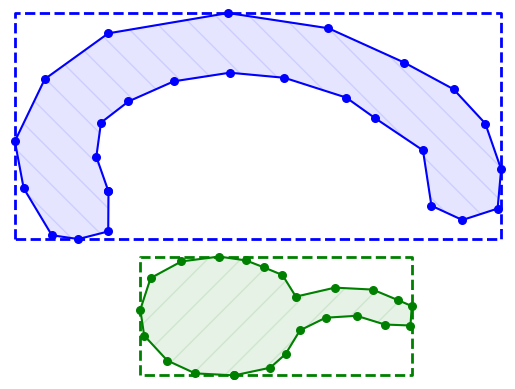
\includegraphics[width=4.25cm]{images/bbox_none.png} }}
    \qquad
    \subfloat[]{{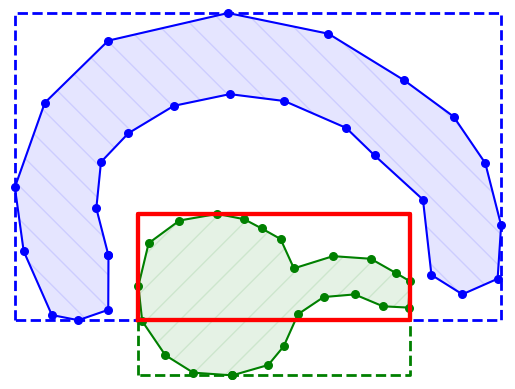
\includegraphics[width=4.25cm]{images/bbox_partial.png} }}%
    \qquad
    \subfloat[\label{fig:fully_contained_bb}]
    {{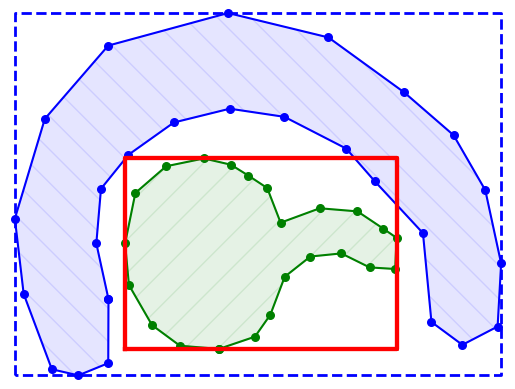
\includegraphics[width=4.25cm]{images/bbox_inside.png} }}%
    \caption{Possible intersection cases between bounding boxes. The common bounding box is in red. \textbf{(a)}: None, \textbf{(b)}: Partial, \textbf{(c)}: Contained.}
    \label{fig:bbi}
\end{figure}

The methods below are based on the assumption that, for the domain of maps, line segments of geometries should not self-intersect, and any occurrence of such is considered an error \cite{self_intersection}. Therefore, if there exists a crossing between any two line segments, it can be concluded that an intersection exists between the two different geometries.


\label{initialAlgo}
\subsection{Initial Intersection Algorithm}

The first algorithm to calculate the predicate intersection is presented below. The algorithm is constrained to not include line segments without an endpoint in the common bounding box and assumes that no shape is fully contained. Due to the constraints being violated in certain intersection contexts, the algorithm described in Section \ref{sect:chkintersect} is instead implemented in FPDE  to allow for more use cases.

\begin{figure}[htbp]
    \centering
    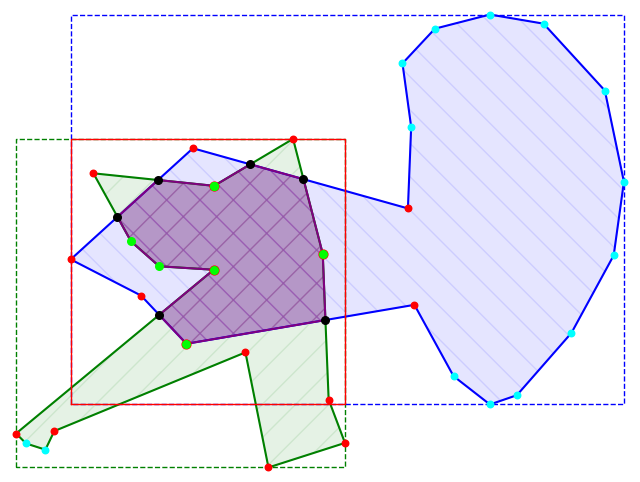
\includegraphics[width=8.5cm]{images/intersection_v1.png}
    \caption{Working case for the first intersection method. Green vertices are part of the intersecting shape, black are \textit{intersection points}, red are unnecessarily decompressed, and cyan are ignored.}
    \label{fig:intersectv1demo}
\end{figure}

When investigating two different geometries, the only area in which they can co-exist is inside the overlap of the bounding boxes. Consequently, an intersection between the two can only occur inside this overlap. The first method tries to avoid local decompression of points outside this area using the following steps:

\begin{enumerate}
    \item Check if the two geometries' bounding boxes overlap; if yes, continue to (2), else return False.
    \item Extract all the points within the overlap of the bounding boxes and add them to a set \textit{S}.
    \item Create a set \textit{L} of all line segments with an end point in \textit{S}.
    \item Check for intersections between any two line segments from each shape.
    \item  Return True if an intersection is found in (4), otherwise return False.
\end{enumerate}

Step (1) is trivially checked using the \textit{separating axis theorem}, while extracting all the points inside the overlap of the bounding boxes in (2) is more involved and requires additional data in the format header. One solution to finding the points is to store two sorted indices lists for the points based on their respective x- and y-value in the compressed format. Since an index can be saved with a maximum of $\lceil \log_2(n) \rceil$ bits, where $n$ is the total number of points in the geometry, the additional per-point overhead is relatively small. 

When the indices lists sorted by x- and y-values are accessible, the points inside the intersecting area of the bounding boxes can be found in $\mathcal{O}(\log_2(n)) \cdot T(random\_access)$ time using four binary searches over the sorted indices list for each geometry. The binary search finds the closest points to each of the bounding box overlap's perimeters; denoted as $x_{left},\ x_{right},\ y_{bottom},\ y_{top}$. When these points are found, the points with x-values between the range $(x_{left},\ x_{right})$ and $(y_{bottom},\ y_{top})$ can be extracted by slice indexing the sorted index lists and taking the set intersection. The last step in extracting all points within the area is to use random access, described in Section \ref{Random_access}, to get the actual points corresponding to the remaining indices.

Step (3) of the algorithm creates all line segments with the points found in (2) over the set of points in the bounding box overlap. Lastly (4) can utilize the \textit{sweep lines algorithm} to efficiently find any line segment intersection, as opposed to comparing each line segment of each geometry with each other.

Figure \ref{fig:intersectv1demo} demonstrates the algorithm. Only the vertices on a segment which is inside the common bounding box are decompressed, with some exceptions during the binary searches.

\begin{figure}[htbp]%
    \centering
    \subfloat[\centering The red intersection points are not found.]{{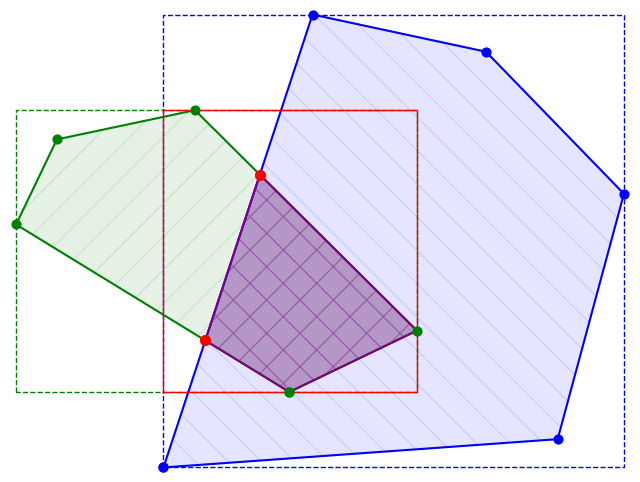
\includegraphics[width=6.9cm]{images/v1_fail_line.png} }}%
    \qquad
    \subfloat[\centering Intersection with no crossing line segments.]{{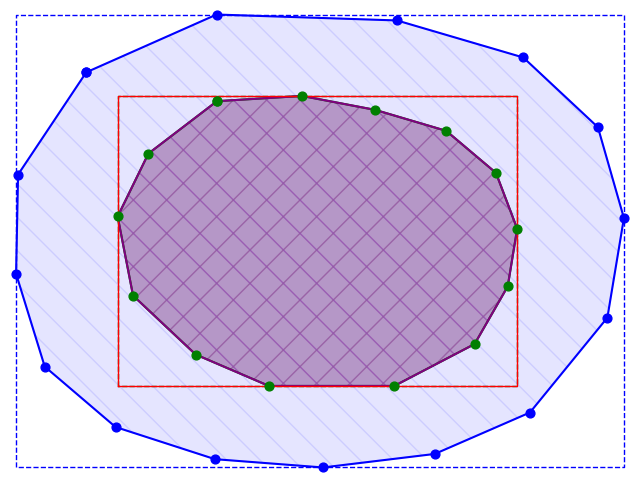
\includegraphics[width=6.9cm]{images/v1_fail_contains.png} }}%
    \caption{Example of failing cases for the first intersection method.}%
    \label{fig:bbFail1}%
\end{figure}

This algorithm works efficiently since it usually operates on a fraction of the geometries' points and line segments. However, it is limited in the sense that certain cases are not processed correctly. Since the algorithm is centralized around creating line segments with any endpoint inside the bounding box overlap, the algorithm does not consider line segments that cross the geometry bounding box overlap area but have both endpoints outside it. Another case in which the algorithm can fail is when the geometries' line segments never cross each other, but one is entirely contained in the other. Figure \ref{fig:bbFail1} shows an example of such cases. Due to these constraints, additional algorithms supporting more use cases for \textit{Is Intersection} and \textit{Intersection} are proposed below.





\subsection{Chunk Based Intersection}
%(Binärt) träd för att indexera baserat på plats. Plats -> index/offset
%Även hur vi lagar och parsear dessa på bästa sätt.  Behöver vi läsa in hela trädet?
\label{sect:chkintersect}
By utilizing the automatic chunking of FP-delta, the implementation for intersection can be improved further. Below, a method that uses the chunk's bounding boxes for reducing the size of the required local decompression is presented.
\\\\
Since the chunks contain a continuous sequence of points, the spatiality of the chunks is localized. As seen in Figure \ref{fig:chunks}, the bounding boxes of the chunks divide the geometry into a set of mostly non-intersecting rectangles. By examining the bounding boxes of the chunks, the relevant chunks which are within the common geometry bounding box can be extracted.

\begin{figure}[htbp]
    \centering
    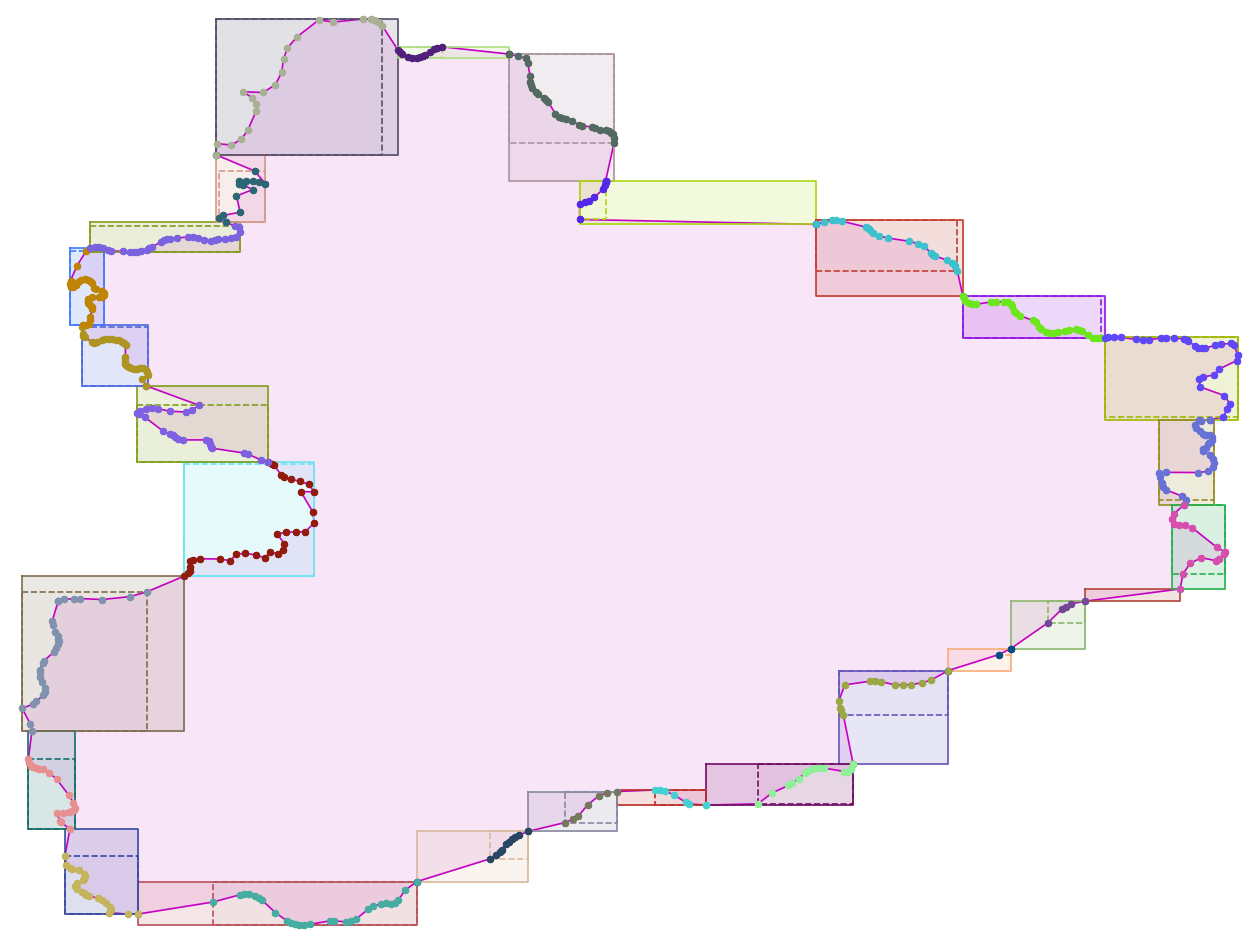
\includegraphics[width=10cm]{images/chunks.png}
    \caption{Bounding boxes of the chunks when including the first point in the following chunk. Dashed line is the bounding box if only containing the points within each chunk.}
    \label{fig:chunks}
\end{figure}

When all chunks within the bounding box have been found, additional filtering is applied to reduce the number of decompressed chunks. As outlined in Section \ref{initialAlgo}, the \textit{separating axis theorem} can be used to check if two bounding boxes overlap. This theorem is applied between the chunk-local bounding boxes between each of the geometries. If a chunk is found to have no bounding box overlap to any of the chunks from the other geometry, assuming no self-intersecting geometries, an intersection point can not exist on the segments in that chunk. For \textit{Is Intersection}, there is no meaning in decompressing such a chunk, but for \textit{Intersection}, it cannot be dismissed yet. In \textit{Intersection}, the segments in a chunk that does not have a bounding box overlap with any of the chunks in the other geometry might still be a part of the output polygon, as they may link the chunks containing intersecting segments. Due to this, these chunks are marked with mock segments and are lazily decompressed at a later stage when it is definite that its segments will be used.

Once the filtering has been completed, the chunks are decompressed and all points within them are used to form line segments. Each chunk forms one linestring consisting of the chunk's line segments. Furthermore, all linestrings filtered from geometry $g_1$ are checked for intersection with all linestrings filtered from  geometry $g_2$. This procedure results in a set $S$ that contains the intersecting points. If $S \neq \emptyset$ then there exists an intersection between the shapes, otherwise additional steps are required to determine the intersection status.

\subsubsection{Fully Contained}
\label{sec:fully_contained}
As stated in the previous algorithm, when one shape is fully contained within the other, there is an intersection between the shapes, even though there are no intersecting points between the shape's line segments. By looking at the relationship between the shapes' global bounding boxes, it can be determined whether it is possible for one shape to be fully contained within the other. Namely, in order for a shape to be fully contained, its bounding box must also be fully contained within the other shape's bounding box. The reason for this is that since the shapes are contiguous (if not dealing with multipolygons), there must exist a path between the points spanning the bounding box. This path will be outside the bounding box of the other shape, and since the geometry is at least as small as its bounding box it can be concluded that the shape cannot be fully contained.

\begin{figure}[htb]
    \centering
    \includegraphics[width=10.75cm]{images/intersecting_ray.png}
    \caption{A query where a ray, visible as the dotted red line, is used to determine intersection. Only the chunks in black (red and green points) are decompressed for the complete query.}
    \label{fig:intray}
\end{figure}

\label{sec:pointinshape}
However, if the bounding box $bounds(g_1)$ is fully contained in $bounds(g_2)$, further evaluation is needed. Since there are no point intersections, the whole geometry is either inside the other shape, or completely outside (but still within its bounding box), as in Figure \ref{fig:fully_contained_bb}. The \emph{crossings test} can be used to determine whether a point is within a shape \cite{polygonalgos}. The test works by sending a ray from the point along an axis, and counting the number of crosses over the shape. If the number is odd, then the point is within the shape, otherwise outside. By picking a random vertex from $g_1$ and performing the crossings test between the vertex and $g_2$, it can be determined that if the point is inside $g_2$, then $g_1$ is fully contained within $g_2$ and $g_1$ is the resulting intersecting shape. An example of an intersection query where the test is performed can be seen in Figure \ref{fig:intray}.


Implementation wise, the ray test in FPDE is implemented by constructing a linestring between the point and the other shape's bounding box. The direction is chosen such as to minimize the length of the line segment. The above steps for finding the intersecting points are then executed for $g_2$ with the common bounding box being the linestring. The number of intersecting points is then equal to the number of crossings.

\begin{figure}[htb]
    \centering
    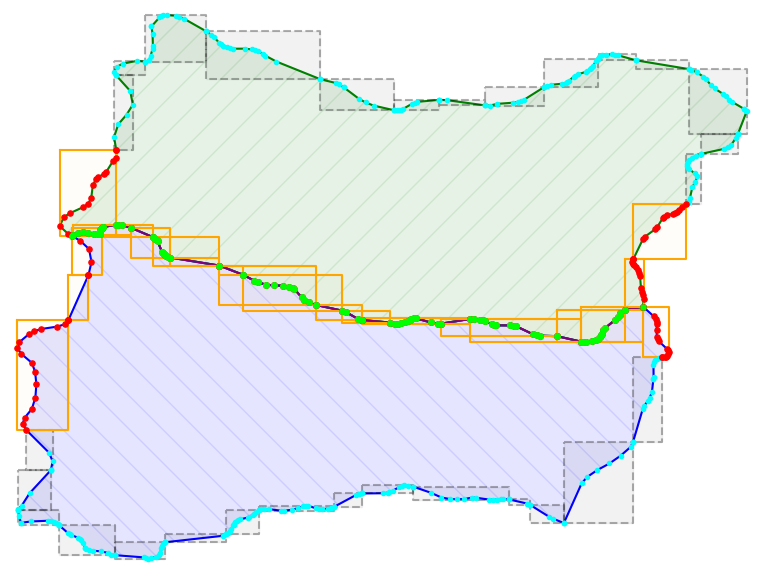
\includegraphics[width=13cm]{images/intersection_world.png}
    \caption{One example from the \emph{Admin Borders} dataset. Only the chunks in black (red and green points) are decompressed. Green vertices are part of the intersecting shape, red vertices are unnecessarily decompressed, and cyan vertices are ignored. }
    \label{fig:intworld}
\end{figure}

As seen in Figure \ref{fig:intworld}, the algorithm has the benefits of local decompression being restricted to the chunks that overlap between the geometries and that are within the common bounding box, with the possible exception of chunks that cross the ray used to test for fully contained shapes. But it also has drawbacks, such as requiring the bounding boxes of the chunks to be quickly accessible and that all points within the overlapping chunks are decompressed.

\starsubsection{Quadtrees for Chunk Based Spatial Indexing}
\label{sec:quadtreechunk}
This section introduces a storage-efficient alternative to spatially indexing chunks. Due to time constraints, implementing the indexing is left as future work.

The overhead for the method presented above comes from the need to find all the chunks possibly involved in an intersection. In the FPDE implementation, all chunks' bounding boxes are stored as full coordinates, adding an additional four floating-point coordinates per chunk to the compressed file, and finding the relevant chunks is done through a linear search. 

Section \ref{sec:quadtreeapproximation} describes how the chunks' bounding boxes can be approximated by utilizing a quadtree. With this approach, the bounding boxes of the chunks are essentially snapped to the smallest quadrant in the quadtree in which they are fully contained.

\begin{figure}[htbp]%
    \centering
    \subfloat[\centering Chunks belong to the smallest quadrant in which they are fully contained.]{{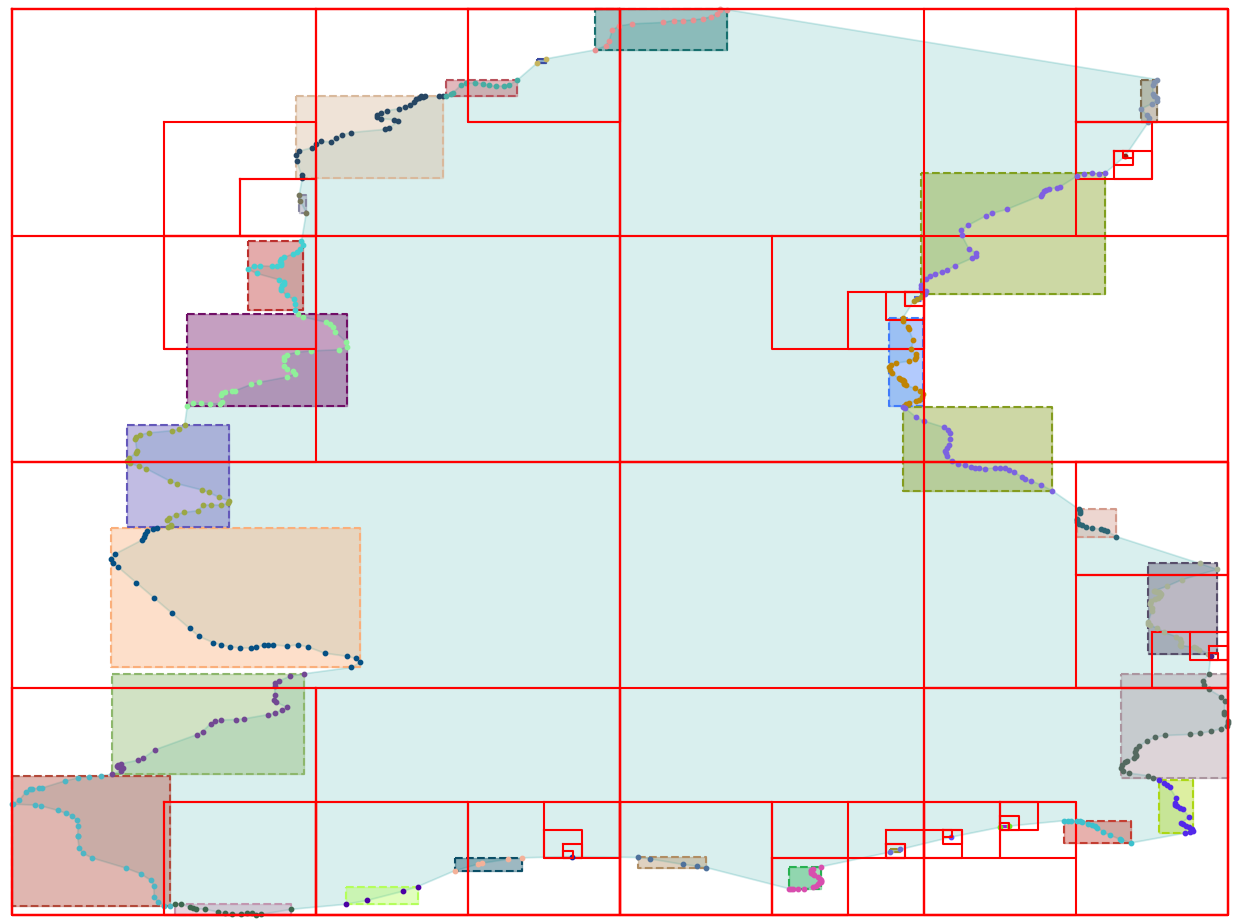
\includegraphics[width=6.9cm]{images/quadtree_contained.png} }}%
    \qquad
    \subfloat[\centering Chunks can belong to multiple quads.]{{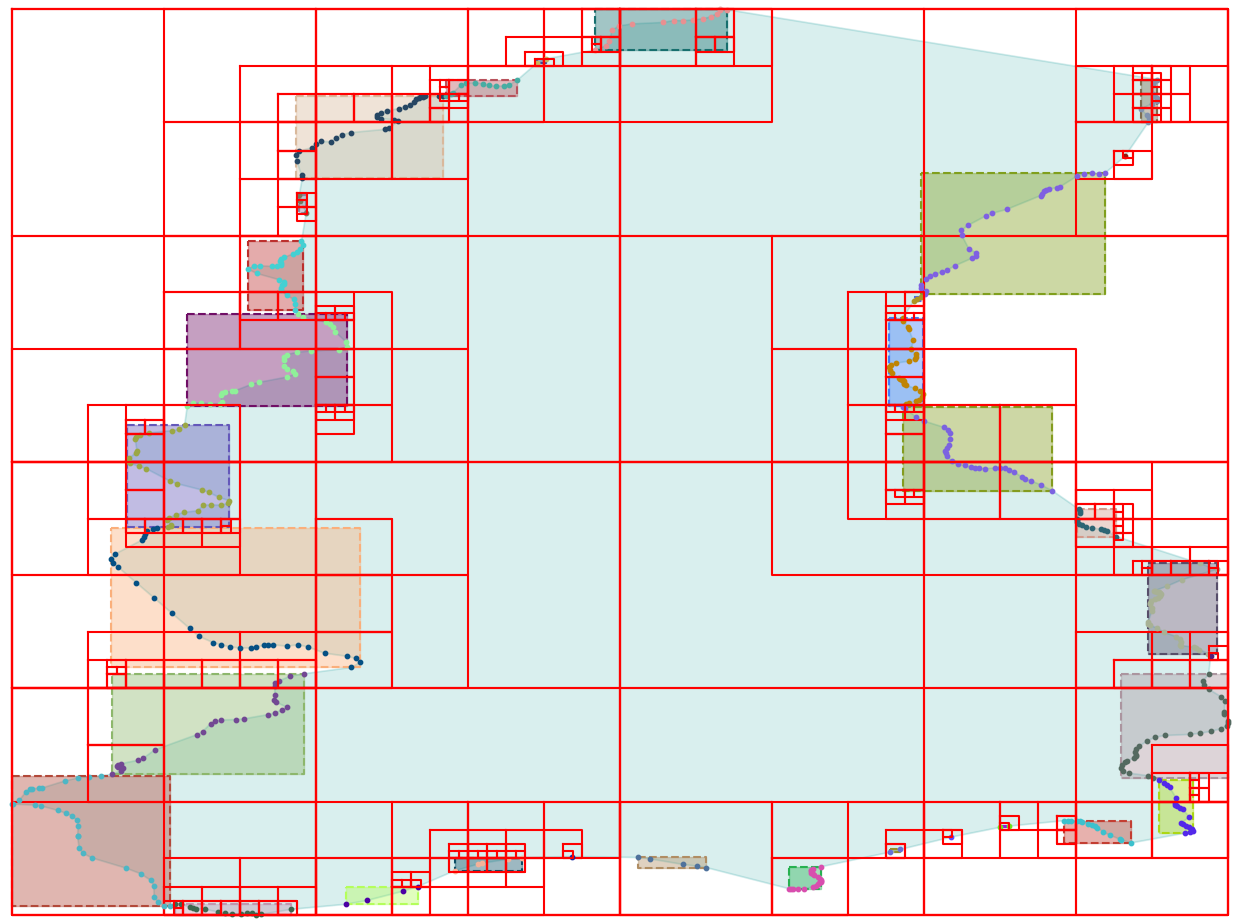
\includegraphics[width=6.9cm]{images/quadtree_min.png} }}%
    \caption{Two configurations of using quadtrees to spatially index chunks.}%
    \label{fig:chkbboxquad}%
\end{figure}

As seen in Figure \ref{fig:chkbboxquad}(a), the quadtree introduces a hierarchy of bounding boxes. The hierarchy allows for a reduction in storage overhead since encoding the bounds of the chunks is done through the tree structure, and the tree structure likely requires less storage space as opposed to storing the coordinates in full. Using a quadtree makes it possible to calculate the bounds of the chunks based on the shape's global bounding box and the position of the quadrants containing the chunks.

Furthermore, since the tree is hierarchically structured, intersection-filtering can be performed on multiple zoom levels. The quadtree can either be based on the geometry's bounding box or on a \emph{global grid}. In both cases, the traversal of the nodes in geometry $g_1$ can be stopped early if a quadrant in $g_1$ only intersects with leaf nodes without chunks in geometry $g_2$. Since if all the intersecting quadrants from $g_2$ are empty leaf nodes, there can be no chunks in those quadrants, and thus no line segments can possibly intersect between the shapes in $g_1$'s quadrant. Expanding the quadrant's subtree further is unnecessary.

% In terms of space, the required size to store the chunks $C$ in a quadtree with nodes $Q$ is:
% \begin{equation}
%     S = 4 \cdot \#(Q) + \#(C) \cdot len(\#(C)) = 4 \cdot \#(Q) + \#(C) \cdot \left \lceil{\log_2{(\#(C))}}\right \rceil 
% \end{equation}


One problem with assigning each chunk to one quadrant only is that the approximation errors may be big. As seen in Figure \ref{fig:chkbboxquad}, allowing chunks to be part of multiple quads results in a more detailed tree. However, this comes at the expense of storing more nodes.

\subsection{Constructing the Intersecting Shape}
Implementing the intersection operation which returns the resulting shape is an involved task, largely due to the numerous possible combinations of shapes and corner cases. The method presented below is an adaptation of the \emph{Weiler Atherton} and \emph{Greiner–Hormann} polygon clipping algorithms, extended to work with spatially separated chunking and linestrings.

\begin{figure}[htbp]
    \centering
    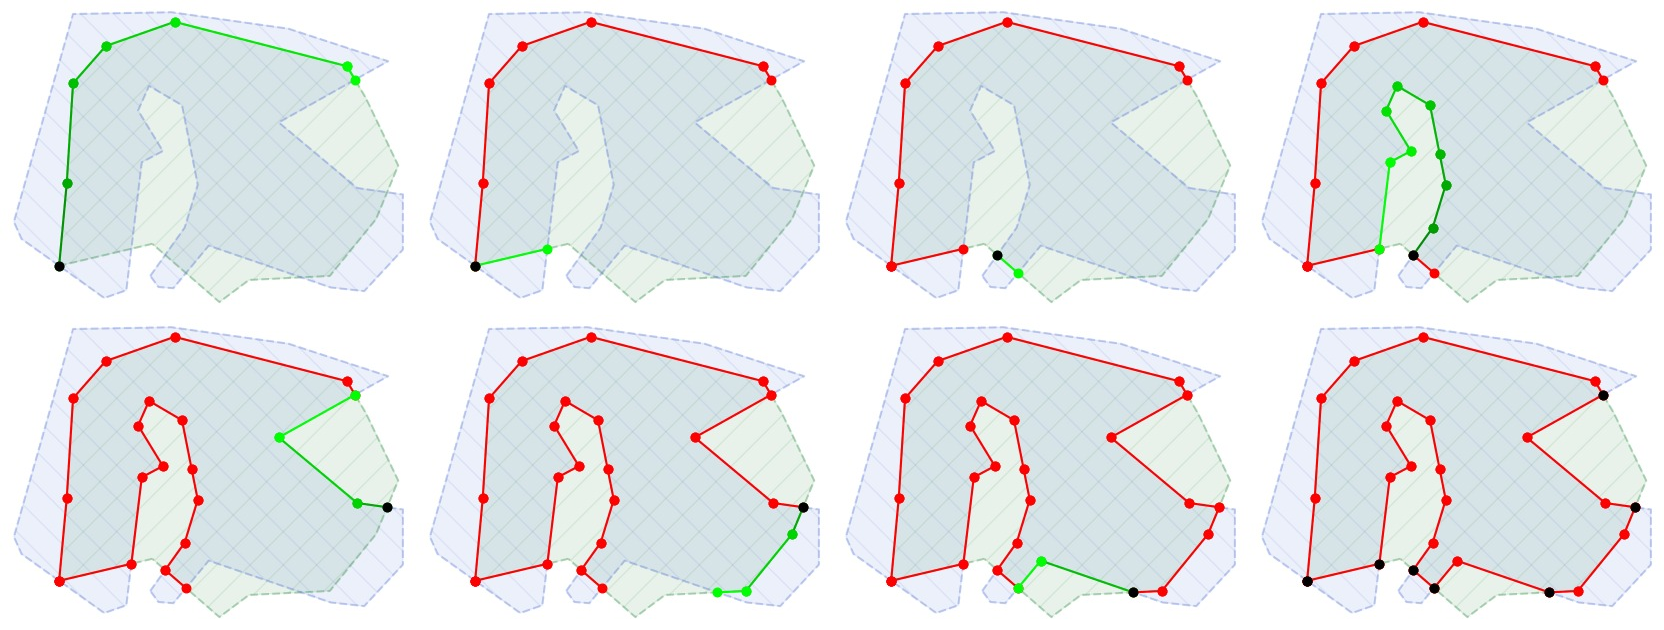
\includegraphics[width=15cm]{images/intersecting_shape.png}
    \caption{Finding the intersecting shape illustrated. Black vertex is the current \emph{intersection point}, green is the current path (traversing from dark to light), and red is the resulting shape.}
    \label{fig:shapegen}
\end{figure}

The steps for the implemented algorithm are the following (illustrated in Figure \ref{fig:shapegen}):
\begin{enumerate}
    \item The common bounding box is calculated. If no common bounding box exists, then the resulting shape is the None-shape. Otherwise, all chunks inside the common bounding box are found.

    \item Chunks with a bounding box that overlaps any of the chunks of the other geometry are immediately decompressed, while the rest are subject to lazy decompression.
   
    \item All segments within each decompressed chunk are merged into a linestring. The linestrings of overlapping chunks are pairwise, one from each shape, checked for intersection. Two dictionaries are created, one that enables finding all segments which cross a given intersection point, while the other is used to go in the other direction, i.e., retrieving all intersecting points which lie on a segment.

    \item Create a set $S = \{ intersecting\ points \}$. One intersection point $c_i$ is removed from $S$ and the valid edges from $c_i$ are traversed and added to the resulting shape. The traversal is stopped when encountering another intersection point. The procedure is repeated until $S = \emptyset$.

    This step can be implemented by first calculating the possible paths from $c_i$. At most four possible paths can exist since it is assumed that holes do not lie on the polygon border, and that there are no self-intersecting shapes. The paths are, for both shapes, traversed in both directions originating from $c_i$. Since at most two of the four paths are valid, the invalid paths are removed by verifying that the midpoint of the paths' first segment is within both shapes, using the \emph{crossings test} as explained in Section \ref{sec:pointinshape}. By traversing both directions, it is ensured that if the resulting shape is a linestring, that is, if no closed path is formed, then both ends are discovered.

    When the resulting shape is a polygon, both traversal directions can reach all points, and thus two paths can share the same edge. To avoid unnecessary calculations and duplicate segments in the final shape, it is also verified that the first segment in the path has not yet been visited.

    \item As explained for the predicate operation in Section \ref{sec:pointinshape}, intersection can occur even though there exist no intersecting points between the linestrings. In that case, the contained shape is returned.
\end{enumerate}

When verifying the paths, it is also verified that no two paths from one $c_i$ are parallel. This is done to avoid adding identical segments when two shapes share an edge.


%https://books.google.se/books?hl=sv&lr=&id=CCqzMm_-WucC&oi=fnd&pg=PA24&dq=shape+check+if+point+is+inside&ots=mvns05NIbe&sig=xaJJmCNMv9oP6BG4n14shw6zi1A&redir_esc=y#v=onepage&q=shape%20check%20if%20point%20is%20inside&f=false


% Bounding Boxes för chunks
% Läsa de chunks som är aktuella (undvik andra) i den gemensamma bounding boxen
% Packa upp dessa för finare evaluering
% Specialfall fully contained: skicka stråle
% C^2 jämför varje chunk med varje chunk
% Potentiell improvement med quadtree




% As mentioned above, geometries do not self-intersect, and any line segment crossing implies that the two geometries containing those line segments intersect. Looking at two geometries the only area they can possibly co-exist is the overlap of the bounding boxes which also implies any co-existing of line segments. Therefore intersection of two geometries can only occur inside this overlap.


% The first method for \textit{IsIntersection} tries to extract every point inside the area where line segment crossing can occur. Since the overlap of the bounding boxes is the only area where the two geometries can co-exist, an initial attempt is to extract all the line segments between points inside that area and their neighbours.

% Referring to \ref{fig:bbi}\textbf{(b)}, it can trivially be concluded that such intersecting line segments can only occur in the overlap of the geometries' bounding boxes and 


% The method for intersection Since we want to locally decompress as little information as possible, one intuitive method to check for intersection is to only use points inside the overlap of the geometries bounding boxes
% Now when the more interesting points, as seen in \ref{fig:bb}\textbf{(b)} are extracted, and local decompression has been done on those, the two operations \textit{IsIntersecting} and \textit{Intersection} take different routes. 




% For the domain of maps, line segments of geometries should not self-intersect, and any occurrence of such is considered an error \todo{källa}. With that assumption in mind, any pair of line segments from different geometries intersecting means that one geometry enters the interior part of the other. \todo{Nämna hur man kan använda line sweeps, bör skivas om i teorin innan} For \textit{IsIntersecting}, any occurrence of such line segment crossing leads to a return value of \textit{True}, representing that an intersection does occur. If no such pair exists, the conclusion can be drawn that an intersection does not occur. 
%FRÅGAN ÄR OM MAN SKA BÖRJA SKRIVA OM FPDE detaljerad implementaion med binary search och hur vi sparar sorterade listor redan här. Även lite osäker om du tänkte att denna mer detaljerade delen skulle vara här, men tänkte att det oavsett kommer behöva skriva någon gång



\section{Optimizing the Compression Ratio}
In this section, additional ideas and implementations that extend FPDE to improve the compression ratio are discussed. First, the alternatives between different formats for representing the coordinates are presented, followed by entropy encoding of the deltas.

\subsection{Floating-Point Coordinate Representation}
\label{sec:delta_mod}
As described in Section \ref{section:fpd}, the standardized way to represent floating-point values is according to the IEEE 754 standard. The standard supports either 32 or 64-bit precision, where high-precision coordinate values can be stored losslessly using the latter, as in the WKB format. Maps data may consist of coordinates with a precision below the need for 64-bit double precision. When this is the case, reducing the number of bits used to represent the floats will decrease the overall size of the geometry format. Two floating-point coordinate representations specific to maps data are presented below.

\subsubsection{Variable Precision Float}
\begin{figure}[htbp]
    \centering
    \includesvg[width=13cm]{images/varfloat.svg}
    \caption{Structure of the \textit{variable precision float} format with a minimal exponent allowing an integer part between \(\pm 180\).}
    \label{img:variable_precision}
\end{figure}

The structure for representing floating-point values proposed in Figure \ref{img:variable_precision} is a modification of the IEEE 754 standard, with a variable exponent and mantissa size. The perk of having variable exponent and mantissa bit-lengths is that it allows for domain-specific optimizations.

For instance, the standard exponent size of IEEE 754 with 64-bit precision allows values ranging between $\pm 9\ 007\ 199\ 254\ 740\ 992$. While for the domain of maps, coordinates are within the range of $\pm 180$, so there is no need to use an exponent part that allows integer ranges outside of that. Therefore, it makes sense to either remove those bits to lower the format size or dedicate some of the unnecessary exponent bits to the mantissa part for a higher floating-point precision.

OpenStreetMap data coordinates use at maximum seven decimal points. Therefore, using the \textit{variable precision float} format with a 4-bit exponent and 32-bit mantissa is enough to represent all coordinates for such data, resulting in a decrease of 27 bits per coordinate from the original 64-bit representation. If full double precision is required, the decrease of bits in the exponent part reduces the total size by 7 bits.


\subsubsection{32-Bit Integer Decomposed Coordinate}
\label{32-bit}
An alternative format that also takes advantage of the limited range of the integer part of the floating-point values in the domain of geographic coordinates is \textit{32-bit integer decomposed coordinate}, illustrated in Figure \ref{img:intdecompflow}. The encoding of the format is performed by adding 180 to the floating-point value, to convert the coordinate to the positive space, followed by concatenating the integer and decimal part into one large unsigned integer value. The integer value is then converted to its corresponding bit sequence.

\begin{figure}[htbp]
    \begin{adjustwidth}{15pt}{}
        \includesvg[width = 400pt]{images/int_decomp.svg}
    \end{adjustwidth}

    \caption{Illustration of converting from floating-point value to a 32-bit integer decomposed coordinate sequence.}
    
    \label{img:intdecompflow}
\end{figure}

The latitude and longitude values of geographic coordinates range between \(\pm 90\) and \(\pm 180 \), respectively \cite{dec_deg}. Thus, the number of possible values for the longitude, when using \(X\) decimals of precision, is \(2 \cdot 180 \cdot 10^{X}\). This is strictly greater than the amount of possible combinations of latitude values with the same decimal precision. For this expression to fit in a 32-bit integer, the precision of the coordinate can not transcend seven decimal points, or else they need to be truncated in a compression-lossy manner. However, since the seventh longitude decimal point corresponds to a real-time accuracy of 1.11 cm at the equator and an even higher accuracy when deviating from it \cite{dec_deg}, the loss of precision above this limitation may be considered acceptable. For instance, as previously noted, OSM operates on coordinate points with up to seven decimal points of precision \cite{osm_precision}, which supports the adequacy of the format for general-purpose mapping applications.
\\\\
When calculating the deltas for coordinates in the IEEE 754 format, only the exponent and sign parts are usually similar between the bit sequences of two adjacent values. Consequently, only those bits systematically cancel out. The mantissa, which covers a great fraction of the bits in IEEE 754, is still generally significantly different.

By using 32-bit integer decomposed coordinates instead, the number of leading zeros in the zigzag encoded deltas is inversely proportional to the distance between the coordinates, and hence the deltas have the possibility of being significantly smaller. However, it is worth recalling that using 32-bit integer decomposed coordinates is not as general as using the IEEE 754 format, as the coordinates are limited to seven decimal points.


\subsection{Entropy Encoding of Deltas}
When using delta encoding, a distribution of the different delta values emerges. If the distribution is not uniform, there is an indication of possible entropy encoding, where more frequent deltas are encoded with fewer bits than infrequent ones. This section presents how Huffman and Golomb-Rice encoding, explained in Section \ref{section:huff}, can be applied to the deltas in the format. %In figure \ref{img:entropy}, it can be seen, intuitively, how the deltas can create a distribution of values.

% \begin{figure}[H]
%     \begin{adjustwidth}{20pt}{}
%         \includesvg[width = 400pt]{images/entropy distribution.svg}
%     \end{adjustwidth}

%     \caption{An illustration how delta values create a distribution which can be entropy encoded}
%     \label{img:entropy}
% \end{figure}

\subsubsection{Huffman Encoding}
Huffman encoding maps a symbol to a bit sequence, and in the context of FPDE each zigzag encoded delta is a symbol.

One way to create a Huffman encoding tree is to use the frequencies of the delta symbols over all geometries in a dataset. However, if the Huffman encoding tree is based on multiple geometries with different delta bit-lengths, a suboptimal Huffman tree will be created since the character space contains deltas of all the combined bit-lengths. 

Instead, as the geometries in FPDE have different but fixed delta bit-lengths, a more efficient approach is to construct a set of smaller Huffman trees, each built with deltas of equal bit-length. This strategy avoids using a Huffman tree where certain values cannot occur because of the fixed delta bit-lengths of the geometries. Furthermore, the frequency distribution of the deltas may vary depending on the specific bit-length involved.

\subsubsection{Golomb-Rice Encoding}
Similarly to Huffman encoding, Golomb-Rice encoding can be used to decrease the size of the delta values. As for Huffman encoding, the possible delta values are used as symbols in the encoding. Golomb-Rice encoding performs particularly well when the delta values are clustered around small values and if the frequency decay follows a geometric distribution.

The advantage of Golomb-Rice encoding compared to Huffman encoding is that the overhead is lower. While Golomb-Rice encoding only requires the parameter $k$ to be saved, Huffman encoding requires the entire Huffman tree to be stored, either locally in the geometries or globally as a library variable. 

A suitable value for the parameter $k$ can be calculated using Equation \ref{eq:rice_form}. 


% \todo{lägg till pred functions efter redovisning}
%\subsection{Predictor Functions}
%which use the surrounding context to estimate the deltas.